\chapter{\system{}: valutazione} \label{chap:valutazione} % 6

% Questo capitolo delinea gli obiettivi e la strategia adottata per valutare il sistema. Successivamente, vengono descritti l'ambiente sperimentale, i campioni selezionati per i test e i criteri utilizzate per la valutazione. Infine vengono presentati i risultati ottenuti e si discutono i principali risultati emersi.

\section{Obiettivi e criteri} % 6.1
% \subsection{Strategia di validazione} % 6.1.1

Lo scopo generale della valutazione del sistema è quello di determinare il grado di maturità raggiunto, così da valutarne l'effettiva applicabilità nel contesto reale per cui è stato progettato e stabilire se il suo impiego possa risultare concretamente vantaggioso. La valutazione del sistema \system{} condotta in questa tesi si concentrerà su due obiettivi principali.

Il primo obiettivo, di carattere preliminare e meno rilevante, consiste nel verificare la correttezza funzionale del sistema, accertandosi che i tre moduli principali producano il comportamento atteso nello scenario operativo. In particolare, saranno verificati il corretto funzionamento della pipeline, il suo grado di autonomia e la produzione degli output previsti. Il secondo obiettivo, di maggiore rilevanza e su cui ci si concentrerà maggiormente durante la sperimentazione, consiste nel valutare l'accuratezza dei due output più importanti, i \report{} e il \capture{}, rispetto ai requisiti definiti.

% (\classifier{}, \sreagent{} e \codeagent{})

A tal fine, saranno analizzati i risultati ottenuti su un insieme di campioni di malware sufficientemente vario e rappresentativo dello scenario operativo di riferimento. Per poter interpretare efficacemente e confrontare i risultati ottenuti sarà inoltre necessario definire una metodologia di classificazione che consenta di valutare oggettivamente il grado di complessità dei campioni.

% A tal fine, saranno analizzati i risultati ottenuti su un insieme di campioni malevoli, selezionando quelli maggiormente rappresentativi dello scenario operativo di riferimento. I campioni dovranno essere sufficientemente significativi e presentare un'adeguata varietà, considerando, ad esempio, architetture differenti e campioni sottoposti o meno al processo di stripping. 

In più, dovranno essere utilizzati più LLM, dimostrando l'indipendenza del sistema da uno specifico modello e, soprattutto, analizzando l'influenza delle loro differenti caratteristiche sui risultati ottenuti. Infine, le prestazioni in termini di risorse computazionali e tempi di esecuzione non costituiscono una dimensione di interesse per la seguente valutazione, poiché il sistema non è stato progettato per un utilizzo ad alta frequenza né per operare sotto stringenti vincoli sul consumo di token del LLM.

La strategia di testing proposta prevede una valutazione \emph{end-to-end} progressiva, condotta al termine di ciascun modulo principale della pipeline. Ad eccezione del \classifier{}, la cui valutazione risulta immediata una volta scelti i campioni, per gli altri due moduli è necessario effettuare un confronto con una \emph{ground truth}. Quest'ultima è costituita dalla documentazione relativa al funzionamento e al comportamento dei malware analizzati, insieme ai moduli di cattura effettivamente funzionanti, ed è stata definita con il supporto di un esperto di cybersecurity, SRE e malware analysis.

La valutazione del \classifier{} considera due aspetti distinti, il riconoscimento della natura malevola del campione e l'individuazione della famiglia di botnet a cui appartiene. % basandosi sulla corrispondenza più probabile.

% il componente centrale della pipeline,

La valutazione del \sreagent{} si concentra sulla correttezza e sulla completezza delle informazioni riportate nei \report{}, al fine di determinare l'accuratezza della \reversing{}. In particolare, l'analisi tiene conto sia della presenza delle informazioni attese, sia della loro esattezza, penalizzando eventuali omissioni. Inoltre, per i binari stripped, è necessario valutare quantitativamente e qualitativamente le attività di rinomina svolte, al fine di misurare l'efficacia della \renaming{}.

Infine, la valutazione del \codeagent{} riguarda l'implementazione del \capture{}, verificandone la correttezza funzionale e la coerenza con le informazioni raccolte nei \report{} e con le specifiche fornite attraverso i prompt, i \templates{} e il \textsc{MessageSchema}. % (Comportamento atteso) Gli aspetti puramente stilistici assumono un ruolo secondario.

Come già evidenziato per la difficoltà dei campioni, anche le valutazioni delle informazioni estratte, della rinomina delle funzioni e del codice prodotto richiedono l'individuazione di criteri di valutazione il più possibile oggettivi e riproducibili. % A tal fine, per ciascuno di questi aspetti dovranno essere individuati opportuni criteri di valutazione. 

\section{Configurazione sperimentale} % 6.2

\subsection{Ambiente di esecuzione e LLM} % 6.2.1
% \subsection{LLM} % 6.2.2

Tutti gli esperimenti sono stati condotti utilizzando un computer personale dotato di hardware convenzionale, eseguendo il software sul sistema locale. L'inferenza dei LLM è stata invece eseguita sul \emph{GPU cluster} dell'Università degli Studi di Udine, mediante il software vLLM \cite{vllm2026vllm}.

Per la sperimentazione sono stati selezionati due LLM diversi, \emph{Qwen 3.6 27B} \cite{alibaba2026qwen3.6-27b} e \emph{DeepSeek V4-Flash Preview} \cite{deepseekai2026deepseekv4}. Al fine di rendere più concisi i riferimenti ai LLM, si adotterà l'abbreviazione \emph{Q3627} per il primo e \emph{DS4FP} per il secondo. Nell'\Cref{app:llm} sono descritte in dettaglio le caratteristiche dei LLM utilizzati, le risorse hardware impiegate, le configurazioni di deployment adottate per vLLM e i sampling parameters usati per la presente sperimentazione.

La scelta dei modelli è stata effettuata principalmente sulla base delle risorse computazionali disponibili, tenendo conto delle diverse dimensioni e caratteristiche architetturali dei modelli, nonché delle prestazioni da essi riportate nei principali benchmark pubblici di valutazione, tra cui \cite{artificialanalysis2026aaii}. 

\subsection{Protocollo sperimentale} % 6.2.2

Ciascun campione di malware è stato sottoposto a una singola esecuzione secondo un protocollo sperimentale uniforme che, grazie all'autonomia del sistema durante l'esecuzione, è stato applicato in modo coerente a tutti i campioni. L'analisi è stata avviata manualmente fornendo in input il \binary{} e la \kb{}, mantenuta invariata per tutti gli esperimenti. Il sistema ha quindi eseguito autonomamente le operazioni previste fino al completamento del processo, producendo tra gli output i \report{} e il \capture{}, successivamente utilizzati per la valutazione dei risultati.

\section{Definizione dei criteri di valutazione} % 6.3

\subsection{Complessità del campione} % 6.3.1

Per caratterizzare la complessità di ciascun campione è necessario individuare gli elementi che contribuiscono a rendere più difficoltosa l'estrazione delle informazioni, attribuendo a ciascuno di essi un punteggio proporzionale al grado di complessità introdotta.

A tal fine sono stati individuati i criteri riportati nella \Cref{tab:complexity_criteria}, insieme a una descrizione del loro ruolo e del relativo significato. Ad eccezione del primo criterio, che tiene conto del risultato della decompilazione prodotto dal framework di SRE adottato, tutti gli altri descrivono direttamente caratteristiche e proprietà del malware analizzato. % (malware o binario)

I criteri possono essere di tipo binario, con l'assegnazione del solo valore minimo o massimo, secondo la notazione \(\{min,max\}\), oppure possono assumere valori variabili nell'intervallo \([min,max]\), in funzione della complessità osservata. In entrambi i casi, il punteggio minimo è pari a $0$, mentre quello massimo varia in base alla caratteristica considerata. La complessità del campione, indicata come \emph{Complexity Score}, è definita dalla somma dei singoli punteggi, su una scala da $0$ a $165$. Per convenzione, a un valore maggiore corrisponde una complessità superiore del campione.

% La somma dei valori massimi dei singoli criteri determina un \emph{Complexity Score} teorico massimo pari a $165$.

% Le singole metriche possono assumere valori secondo due modalità. Alcune sono di tipo binario e prevedono esclusivamente l'assegnazione del punteggio minimo o massimo, come nel caso del fingerprinting del sistema compromesso. Altre, invece, possono assumere un valore qualsiasi all'interno dell'intervallo definito, in funzione del livello di complessità osservato nel campione, come per il protocollo di C\&C adottato. In tutti i casi, il punteggio minimo è pari a $0$, mentre il valore massimo dipende dalla specifica caratteristica considerata. La somma dei valori massimi determina un punteggio teorico complessivo pari a $165$, corrispondente al livello massimo di complessità considerato dalla scala proposta.

\renewcommand{\topfraction}{0.80}  % Alloca al massimo l'80/100 della pagina per i float.
\renewcommand{\textfraction}{0.20} % Alloca almeno il 20/100 della pagina per il testo

\begin{table}[t]
    \centering
    \ExecuteMetaData[chapters/T.tex]{complexity-criteria}
    \caption[Criteri di valutazione della complessità dei campioni malevoli]{Criteri di valutazione della complessità dei campioni malevoli e relativi intervalli di punteggio. La notazione $\{min,max\}$ indica che il punteggio può assumere esclusivamente i valori $min$ o $max$, mentre $[min,max]$ indica che può assumere qualsiasi valore compreso nell'intervallo.}
    \label{tab:complexity_criteria}
\end{table}

\subsection{Efficacia della \renaming{}} \label{sec:renaming_criteria} % 6.3.2

Per la valutazione dell'efficacia della \renaming{} è necessario considerare due parametri principali. Il primo, indicato come ${RC}_{\%}$ e definito \emph{Renaming Coverage}, rappresenta la percentuale di funzioni rinominate rispetto al totale delle funzioni presenti nel binario.

\begin{equation*}
    {RC}_{\%} = \frac{N_{fun. \text{ renamed}}}{N_{fun. \text{ total}}} \cdot 100
    \label{eq:renaming_coverage}
\end{equation*}

Il secondo parametro considera invece la qualità dei nomi assegnati e corrisponde alla percentuale di funzioni rinominate alle quali è stato associato un nome semanticamente corretto sulla base del comportamento osservato. Tale valore, indicato nel seguito con ${RA}_{\%}$, viene definito \emph{Renaming Accuracy}.

\begin{equation*}
    {RA}_{\%} = \frac{N_{fun. \text{ correct}}}{N_{fun. \text{ renamed}}} \cdot 100
    \label{eq:renaming_accuracy}
\end{equation*}

Considerando che la strategia adottata per la \reversing{} tende a coinvolgere principalmente le funzioni più rilevanti per l'analisi, escludendo quelle di minore interesse, e che il numero di funzioni presenti nei campioni è generalmente elevato, è difficile aspettarsi valori di ${RC}_{\%}$ prossimi al $100\,\%$. Inoltre, all'aumentare del numero di funzioni rinominate, si può ipotizzare un effetto di \emph{diminishing returns}, per cui il beneficio derivante da ulteriori ridenominazioni tende progressivamente a ridursi.

% Considerando la strategia adottata dal \textsc{SRE Agent} per la fase di rinomina, che procede ricorsivamente a partire dal \texttt{main}, e il numero generalmente elevato di funzioni presenti nei campioni, è difficile aspettarsi valori di ${RC}_{\%}$ prossimi al $100\,\%$. La strategia tende infatti a coinvolgere principalmente le funzioni più rilevanti per l'analisi, mentre le funzioni di importanza minore vengono progressivamente escluse. Ne deriva un effetto di \emph{diminishing returns}, per cui l'incremento del numero di funzioni rinominate produce un beneficio progressivamente minore.

Risulta quindi logico proporre un punteggio composito che unisce i due parametri. Per tenere conto dei rendimenti decrescenti associati a ${RC}_{\%}$, viene applicata una trasformazione logaritmica attraverso la funzione $g$, normalizzata nell'intervallo $[0,1]$ e dove $k>0$ controlla il grado di attenuazione del contributo di ${RC}_{\%}$. Il punteggio finale, indicato con ${RS}_{\%}$ e chiamato \emph{Renaming Score}, è volto a premiare una combinazione elevata di copertura e correttezza semantica.

% La funzione è normalizzata in modo tale che $g(0)=0$ e $g(100)=1$, mantenendo invariati gli estremi dell'intervallo considerato.

\begin{equation*}
    {RS}_{\%} = g({RC}_{\%}) \cdot {RA}_{\%}
    \label{eq:renaming_score}
\end{equation*}

\begin{equation*}
    g(x) = \frac{\log (1+k \cdot \frac{x}{100})}{\log(1+k)}
    \label{eq:logarithmic_transformation}
\end{equation*}

\subsection{Accuratezza della \reversing{}} % 6.3.3

In modo analogo alla valutazione della complessità del campione, è necessario definire i criteri che consentano di misurare l'efficacia e l'accuratezza della \reversing{}, il cui risultato è rappresentato dalla redazione dei \report{}. La valutazione considera quindi la capacità dell'agente di recuperare gli artefatti rilevanti, oltre che di ricostruire il comportamento e la logica di funzionamento del malware. Vengono penalizzate l'introduzione di ipotesi non supportate, la presenza di informazioni incoerenti o discordanti tra loro e la mancata identificazione di artefatti o elementi rilevanti.

% Le metriche considerate fanno direttamente riferimento agli elementi recuperati durante l'analisi, ad eccezione dell'ultima, che invece si concentra maggiormente sull'organizzazione e sulla coerenza delle informazioni riportate nei documenti finali, penalizzando eventuali contraddizioni o incoerenze.

I criteri scelti per la valutazione sono riportati nella \Cref{tab:reversing_criteria}, insieme a una descrizione della loro interpretazione. A ogni criterio può essere assegnato un punteggio compreso tra $0$ e un valore massimo proporzionato alla sua importanza. I punteggi parziali consentono di valorizzare anche ricostruzioni incomplete ma corrette, evitando che un errore finale annulli le informazioni recuperate, a condizione che queste siano sufficientemente corrette e non fuorvianti. L'accuratezza della \reversing{}, indicata come \emph{Reversing Score}, è definita dalla somma dei singoli punteggi, su una scala da $0$ a $100$.

% Per convenzione, a un valore più elevato corrisponde un'analisi più efficace.

% La somma dei valori massimi determina un punteggio teorico complessivo pari a $100$, corrispondente a un'analisi completa e corretta.

\begin{table}[t]
    \centering
    \ExecuteMetaData[chapters/T.tex]{reversing-criteria}
    \caption[Criteri di valutazione della \reversing{}]{Criteri di valutazione della \reversing{}.}
    \label{tab:reversing_criteria}
\end{table}

\subsection{Qualità del \capture{}} % 6.3.4

La valutazione del \capture{} prende in esame l'implementazione prodotta dal \codeagent{} in termini di funzionalità, correttezza e conformità alle specifiche, senza estendersi agli aspetti stilistici del codice. Inizialmente vengono considerati la correttezza sintattica del codice, l'aderenza ai \templates{} forniti e al \schema{}. A questi si aggiungono due ulteriori criteri, a cui è assegnato un peso maggiore in quanto più rappresentativi dell'effettiva funzionalità del modulo. Il primo riguarda il rispetto del protocollo descritto nei \report{}, mentre il secondo riguarda la \emph{human independence}, che valuta l'autonomia del modulo rispetto alla revisione umana, assegnando punteggi maggiori al diminuire delle modifiche necessarie per renderlo operativo.

I criteri considerati sono riportati nella \Cref{tab:module_criteria}, insieme alla relativa descrizione. I primi tre assumono esclusivamente il valore minimo o massimo previsto, mentre gli ultimi due possono assumere anche valori intermedi. La qualità del \capture{}, indicata come \emph{Module Score}, è definita dalla somma dei singoli punteggi, su una scala da $0$ a $100$.

% Il punteggio complessivo è dato dalla somma dei singoli valori, con un massimo teorico di $100$, corrispondente a un'implementazione funzionante e conforme a struttura e comportamento attesi.

\begin{table}[t]
    \centering
    \ExecuteMetaData[chapters/T.tex]{module-criteria}
    \caption[Criteri di valutazione del \capture]{Criteri di valutazione del \capture{}.}
    \label{tab:module_criteria}
\end{table}

\section{Campagna sperimentale} % 6.4

Per la campagna sperimentale condotta nell'ambito di questa tesi, si è deciso di concentrare l'analisi su una singola famiglia di botnet IoT, \emph{Mirai}, selezionando cinque campioni significativi. La scelta non è casuale, visto che, come descritto nella \Cref{sec:mirai}, anche a distanza di dieci anni dalla sua comparsa la famiglia Mirai continua a essere uno dei principali riferimenti nel panorama delle botnet IoT.

% che rispettano i principi precedentemente definiti

% A distanza di circa dieci anni dalla sua comparsa, i malware derivati da Mirai continuano a dominare il panorama del malware IoT, come evidenziato da due fonti indipendenti.

Tale rilevanza è confermata da due fonti indipendenti. Il \emph{Threat Report 2025} di Zscaler ThreatLabz \cite{zscaler2025threatiot} identifica Mirai come la minaccia prevalente, con una quota del 40\,\%, seguita da Mozi e Gafgyt, entrambe con una quota inferiore al 20\,\%. Anche il report \emph{IT Threat Evolution in Q2 2026} \cite{kaspersky2026itthreat}, basato in parte sulle osservazioni raccolte tramite gli IoT honeypot proprietari di Kaspersky, evidenzia la rilevanza di Mirai e segnala al contempo la crescente attività di un'altra botnet nota, Prometei.

% Tale rilevanza è confermata da due fonti indipendenti. Il rapporto del 2025 di Zscaler ThreatLabz \cite{zscaler2025threatiot} indica Mirai come la minaccia prevalente, con una quota del 40\,\%, seguita al secondo e al terzo posto da Mozi e Gafgyt, entrambe con una quota inferiore al 20\,\%. Dati simili, basati sulle osservazioni raccolte tramite gli ioT honeypot proprietari di Kaspersky, sono confermati anche dal report \emph{IT Threat Evolution} \cite{kaspersky2026itthreat} relativo al Q2 2026, che evidenzia parallelamente la crescita dell'attività di un'altra botnet rinomata, Prometei.

% Complessivamente, queste tre famiglie rappresentano la maggior parte dell'attività osservata, superando i due terzi del totale. (Mirai + Mozi + Gafgyt)

\subsection{Dataset dei campioni} % 6.4.1
% \subsubsection{Provenienza}
% \subsection{Descrizione testuale}

Nella tabella \Cref{tab:malware_samples} sono riportate le principali informazioni relative ai campioni selezionati, tra cui i nomi univoci utilizzati per identificarli, e gli hash SHA-256 dei file binari. Come anticipato, tutti appartengono alla famiglia Mirai, sono in formato ELF e risultano \emph{statically linked}; i primi due sono non-stripped, mentre gli ultimi tre sono stripped.

\begin{table}[t]
    \centering
    \ExecuteMetaData[chapters/T.tex]{malware-samples}
    \caption[Informazioni principali sui campioni di malware selezionati]{Informazioni principali sui campioni di malware selezionati per la campagna sperimentale.}
    \label{tab:malware_samples}
\end{table}

Per quanto riguarda la provenienza dei campioni, i primi tre sono stati catturati tramite l'honeypot proprietario del gruppo di ricerca in cybersecurity dell'Università degli Studi di Udine, mentre gli ultimi due sono stati reperiti dal database \emph{MalwareBazaar} \cite{malwarebazaar2026browse}. Attualmente, tutti i campioni sono disponibili su MalwareBazaar e possono essere recuperati direttamente mediante il relativo hash.

\subsection{\emph{Complexity Score} dei campioni} % 6.4.2

Sulla base dei criteri riportati nella tabella \Cref{tab:complexity_criteria}, la tabella \Cref{tab:complexity_scores} riporta la \emph{Complexity Score} associata a ciascuno dei campioni scelto. I punteggi totali, espressi su un massimo teorico di $165$, vengono anche normalizzati in termini percentuali.

\begin{table}[t]
    \centering
    \ExecuteMetaData[chapters/T.tex]{complexity-scores}
    \caption[\emph{Complexity Score} dei campioni del dataset]{\emph{Complexity Score} dei campioni del dataset, assegnate secondo i criteri della \Cref{tab:complexity_criteria}.}
    \label{tab:complexity_scores}
\end{table}

La complessità dei campioni è piuttosto eterogenea, \textsc{hopto} è il più difficile da analizzare (62\,\%), seguito da \textsc{deepsorrow} (56\,\%) e \textsc{marvisxoxo} (50\,\%); \textsc{onboardboat} presenta una difficoltà intermedia (43\,\%), mentre \textsc{ghost} è nettamente il più semplice (23\,\%).

Risulta particolarmente interessante osservare il contributo dei singoli criteri alla costruzione del punteggio complessivo. Alcuni criteri, come la cifratura della tabella delle stringhe  e il parsing non standard dei comandi , sono presenti nella maggioranza dei campioni, mentre altri, ad esempio la gestione delle risposte e la cifratura della connessione, compaiono in uno soltanto. Il campione \textsc{marvisxoxo} combina la maggior parte delle difficoltà considerate, risultando privo solo della registrazione degli attacchi e dei meccanismi di risposta, oltre a essere non-stripped. Escludendo i criteri non legati alle funzionalità e al comportamento del malware, ossia \emph{ghidra\_dbf}, \emph{statically\_linked} e \emph{stripped}, \textsc{marvisxoxo} presenta un punteggio superiore a \textsc{deepsorrow} e \textsc{hopto}, la cui maggiore difficoltà è dovuta principalmente alla registrazione dinamica degli attacchi.

% (\emph{enc\_str}), (\emph{non\_std\_parsing}) + offuscamento dell'endpoint di C\&C (\emph{obfuscated\_cc}) / (\emph{has\_response}), (\emph{enc\_conn})

% Alcuni, come la cifratura della tabella delle stringhe (\emph{enc\_str}) e il parsing non standard dei comandi (\emph{non\_std\_parsing}), sono particolarmente frequenti e sono presenti in almeno quattro dei cinque campioni. Al contrario, la gestione delle risposte (\emph{has\_response}) e la cifratura della connessione (\emph{enc\_conn}) risultano meno frequenti, essendo presenti in un solo campione ciascuna. Il campione \textsc{marvisxoxo} si distingue per la combinazione della maggior parte delle difficoltà considerate, risultando privo soltanto della registrazione degli attacchi e di meccanismi di risposta, oltre a essere non-stripped. Considerando esclusivamente le difficoltà legate al comportamento e alle funzionalità del malware (cioè escludendo i parametri \emph{ghidra\_dbf}, \emph{statically\_linked} e \emph{stripped}), \textsc{marvisxoxo} presenta un punteggio superiore a quello di \textsc{deepsorrow} e \textsc{hopto}. L'elevata difficoltà attribuita a questi ultimi due campioni è dovuta principalmente alla presenza della registrazione dinamica degli attacchi, mentre, per ciascuna delle restanti caratteristiche, \textsc{marvisxoxo} presenta un livello di difficoltà maggiore o uguale.

\section{Risultati sperimentali}  % 6.5

Nella seguente sezione vengono riportati i principali risultati della campagna sperimentale, condotta secondo il protocollo definito e basata sulle valutazioni effettuate attraverso i criteri selezionati.

Ad eccezione della \Cref{tab:classifier_scores}, i risultati sono organizzati in tabelle caratterizzate da una struttura comune. Le colonne seguono un indice gerarchico a due livelli, in cui il primo identifica il campione considerato, mentre il secondo indica il modello LLM utilizzato; le righe riportano invece i criteri di valutazione e i relativi punteggi.

% I risultati sono riportati mediante tabelle caratterizzate da una struttura comune. Le colonne sono organizzate secondo un indice gerarchico a due livelli, dove il primo identifica il campione considerato e il secondo specifica il modello LLM impiegato per l'esecuzione. Le righe riportano i criteri di volta in volta considerati, con i relativi valori, mentre la parte finale della tabella è dedicata ai punteggi complessivi calcolati a partire da questi.

\subsection{Statistiche di esecuzione} % 6.5.1

La \Cref{tab:execution_stats} presenta alcune statistiche relative alle esecuzioni effettuate sui campioni, riportate a scopo puramente informativo e non considerate nella valutazione del sistema.

La metà superiore della tabella riporta il numero complessivo di token utilizzati dalle attività previste dalle \renaming{} e \reversing{} del \sreagent{} e da quelle del \codeagent{}, oltre al totale. Il conteggio è riferito all'intera esecuzione e non distingue tra token di input, che comprendono prompt iniziali e risposte dei tool, e token di output, che includono reasoning, risposte e tool call.

La metà inferiore mostra invece i tempi di esecuzione relativi alle medesime attività. Rispetto al numero di token, la misura dei tempi è maggiormente soggetta a variabilità e quindi meno precisa, pur fornendo una buona indicazione dell'impegno richiesto dalle diverse attività.

\begin{table}[t]
    \centering
    \ExecuteMetaData[chapters/T.tex]{execution-stats}
    \caption[Statistiche di esecuzione del sistema]{
        Statistiche relative ai token utilizzati e ai tempi di esecuzione delle macro-attività del sistema, con distinzione tra quelle previste dalla \renaming{} (\emph{Ren.}), dalla \reversing{} (\emph{Rev.}) e dal \codeagent{} (\emph{Code}).
        % Statistiche relative ai token utilizzati e ai tempi di esecuzione delle macro-attività del sistema. \emph{Ren.}, \emph{Rev.} e \emph{Code} indicano rispettivamente \renaming{}, \reversing{} e \codeagent{}.
    }
    \label{tab:execution_stats}
\end{table}

% La 1a riga ingloba \textsc{Start Mode} e \textsc{Continue Mode}. La 2a riga ingloba \textsc{Renaming Task} e \textsc{Reversing Task}. La 3a riga include \textsc{BotNet} module e \textsc{MessageParser} module.

\subsection{Raccolta dei risultati} % 6.5.2

La \Cref{tab:classifier_scores} riporta i risultati della valutazione del \classifier{}, nella quale è stato verificato che il modulo riconosca la natura malevola dei campioni e ne identifichi correttamente la famiglia di botnet di appartenenza.

\begin{table}[t]
    \centering
    \ExecuteMetaData[chapters/T.tex]{classifier-scores}
    \caption[Risultati della valutazione del \classifier{}]{Risultati della valutazione del \classifier{}.}
    \label{tab:classifier_scores}
\end{table}

La \Cref{tab:renaming_scores} riporta i risultati della valutazione della \renaming{} del \sreagent{}. La valutazione riguarda esclusivamente i campioni stripped, ossia \textsc{deepsorrow}, \textsc{hopto} e \textsc{onboardboat}, mentre \textsc{ghost} e \textsc{marvisxoxo}, essendo not-stripped, sono esclusi. Per completezza, questi ultimi contengono rispettivamente $329$ e $368$ funzioni. Le prime righe della tabella riportano il numero totale di funzioni, il numero di funzioni rinominate e quello delle funzioni a cui è stato assegnato un nome corretto. Da questi valori sono stati quindi calcolati la \emph{Renaming Coverage}, la \emph{Renaming Accuracy} e il \emph{Renaming Score}, secondo quanto definito nella \Cref{sec:renaming_criteria}. Nel calcolo del \emph{Renaming Score}, la funzione $g$ è stata parametrizzata con $k=10$.

\begin{table}[t]
    \centering
    \ExecuteMetaData[chapters/T.tex]{renaming-scores}
    \caption[Risultati della valutazione della \renaming{}]{Risultati della valutazione della \renaming{} del \sreagent{}.}
    \label{tab:renaming_scores}
\end{table}

La \Cref{tab:reversing_scores} riporta i risultati della valutazione della \reversing{} del \sreagent{}. La valutazione è stata effettuata sulla base dei criteri definiti nella \Cref{tab:reversing_criteria}, da cui è stato calcolato il \emph{Reversing Score}.

\begin{table}[t]
    \centering
    \ExecuteMetaData[chapters/T.tex]{reversing-scores}
    \caption[Risultati della valutazione della \reversing{}]{Risultati della valutazione della \reversing{} del \sreagent{}.}
    \label{tab:reversing_scores}
\end{table}

La \Cref{tab:module_scores} riporta i risultati della valutazione dei \capture{} prodotti dal \codeagent{}. La valutazione è stata effettuata sulla base dei criteri definiti nella \Cref{tab:module_criteria}, calcolando infine il \emph{Module Score}.

\begin{table}[t]
    \centering
    \ExecuteMetaData[chapters/T.tex]{module-scores}
    \caption{Coding performance}
    \label{tab:module_scores}
\end{table}

\section{Discussione dei risultati} % 6.6

Per tutte le esecuzioni effettuate, il sistema ha operato in maniera autonoma secondo il flusso previsto, completando le diverse fasi della pipeline senza richiedere interventi manuali. Tale risultato conferma la corretta integrazione dei diversi componenti e consente quindi di passare alla discussione dei risultati ottenuti per i singoli moduli.

La valutazione del \classifier{}, riportata in \Cref{tab:classifier_scores}, è stata necessariamente limitata ai campioni scelti. In tali casi, il \classifier{} si è dimostrato sufficientemente affidabile, visto che non sono stati incontrati errori di classificazione. Una valutazione più completa richiederebbe tuttavia di considerare anche casi limite, utili a verificare il rilevamento di eventuali falsi positivi e falsi negativi e la capacità di distinguere correttamente tra più famiglie di botnet, in particolare con campioni che presentano caratteristiche riconducibili a più di una famiglia. % mediante criteri di accuratezza

A questo punto, per fornire una visione sintetica dei risultati e facilitare il confronto tra i diversi LLM e i campioni, è stato realizzato il grafico a barre mostrato in \Cref{fig:bar_plot}, che a confronto i punteggi complessivi ottenuti nelle tre valutazioni principali.

% \renaming{} e \reversing{} del \sreagent{} e produzione del \capture{} da parte del \codeagent{}.

\begin{figure}[t]
    \centering
    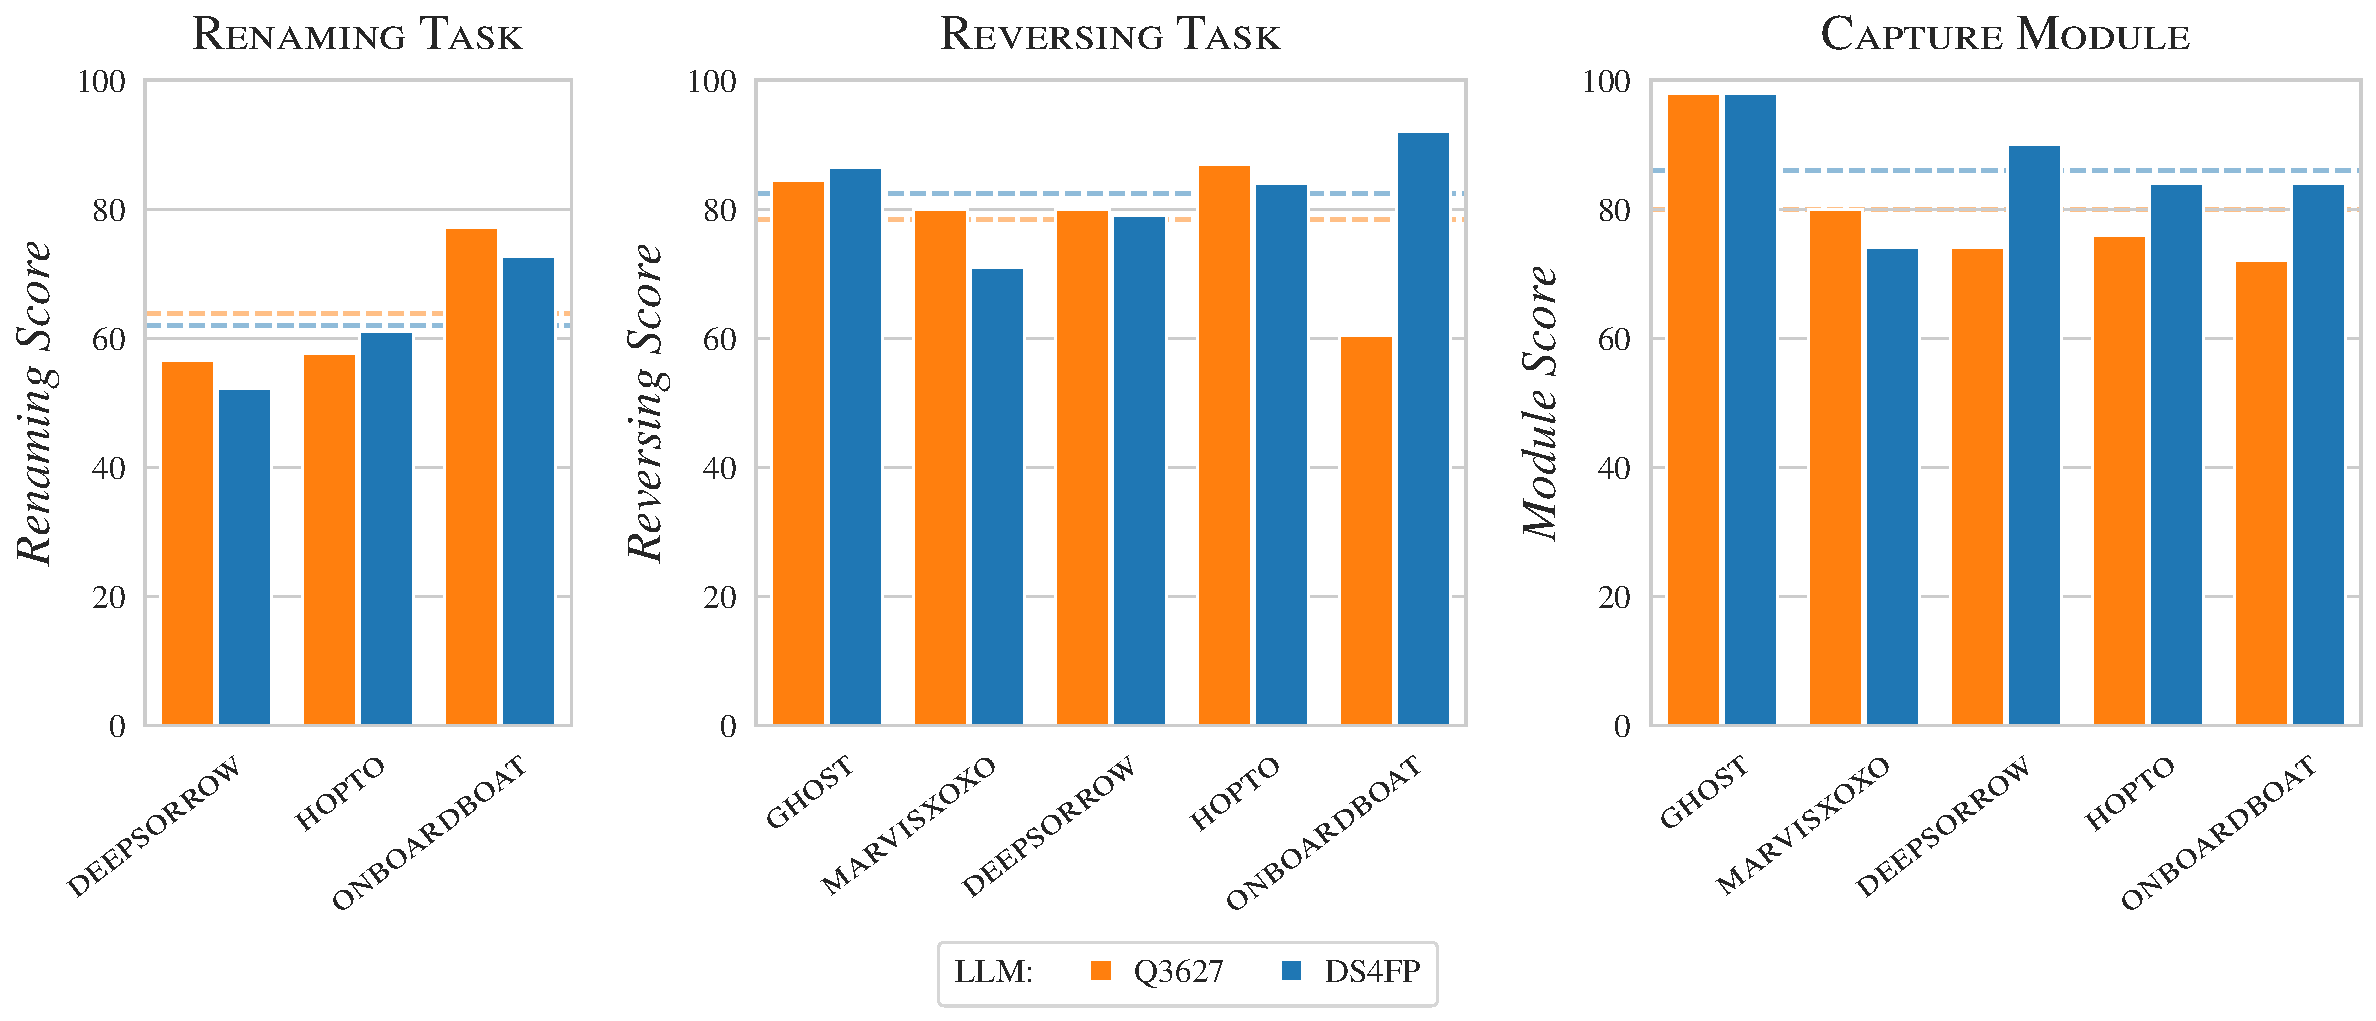
\includegraphics[width=0.95\textwidth]{img/bar_plot.pdf}
    \caption[Confronto tra i punteggi \emph{Renaming Score}, \emph{Reversing Score} e \emph{Module Score} ottenuti]{
        Confronto tra i punteggi \emph{Renaming Score}, \emph{Reversing Score} e \emph{Module Score} ottenuti dai due LLM considerati nelle valutazioni di \renaming{}, \reversing{} e \capture{} su tutti i campioni selezionati. Le linee orizzontali rappresentano la media delle rispettive serie.
    }
    \label{fig:bar_plot}
\end{figure}

A partire dalle statistiche riportate nella \Cref{tab:execution_stats} e dai risultati riassunti nella \Cref{fig:bar_plot}, è possibile confrontare ad alto livello i due LLM nelle attività considerate. Q3627 e DS4FP presentano prestazioni generalmente comparabili, con differenze più evidenti nella produzione del codice, in cui DS4FP mostra un vantaggio più marcato. Anche il consumo di token risulta nel complesso simile, sebbene DS4FP ne utilizzi di più per la \renaming{} e di meno nel \codeagent{}. Per quanto riguarda i tempi di esecuzione, DS4FP risulta costantemente più rapido, con tempi circa dimezzati rispetto a Q3627. Tale differenza è compatibile con le caratteristiche architetturali dei due modelli, in particolare con l'architettura sparsa di DS4FP, che attiva circa la metà dei parametri rispetto a Q3627 \cite{alibaba2026qwen3.6-27b, deepseekai2026deepseekv4}. La vicinanza dei punteggi ottenuti risulta inoltre coerente con alcuni benchmark pubblici. Nell'Artificial Analysis Intelligence Index v4.3.2 \cite{artificialanalysis2026aaii}, che aggrega dieci valutazioni delle capacità dei LLM in vari ambiti, DS4FP ottiene $24$ punti contro i $21$ di Q3627. Nel Terminal-Bench v2.1 \cite{merrill2026terminalbench}, che comprende anche attività simili a quelle di SRE e cybersecurity implementate in questo sistema, DS4FP raggiunge $61.8$ punti contro i $60.7$ di Q3627. I risultati esterni considerati risultano quindi coerenti con gli andamento osservati nel sistema, pur appartenendo a contesti di valutazione differenti.

% Un riscontro analogo si osserva anche nel benchmark Terminal-Bench v2.1 \cite{merrill2026terminalbench}, composto da attività realistiche eseguite tramite terminale, tra cui \emph{extract-elf}, \emph{path-tracing-reverse} e \emph{fix-code-vulnerability}, che coinvolgono ambiti affini a quelli di SRE e cybersecurity considerati da questo sistema. In tale benchmark, DS4FP ottiene 61.8 punti contro i 60.7 di Q3627.

% A A I I v4.2: 33 vs 29
% A A I I v4.3.2: 24 vs 21

\iffalse
https://artificialanalysis.ai/evaluations/artificial-analysis-intelligence-index
https://artificialanalysis.ai/evaluations/omniscience
https://www.tbench.ai/?version=2.1
https://hub.harborframework.com/datasets/terminal-bench/terminal-bench-2-1/latest
https://hub.harborframework.com/tasks/terminal-bench/extract-elf/latest
https://hub.harborframework.com/tasks/terminal-bench/path-tracing-reverse/latest
https://hub.harborframework.com/tasks/terminal-bench/fix-code-vulnerability/latest
\fi

Tornando all'analisi delle singole attività, per la \renaming{} la \Cref{tab:renaming_scores} evidenzia una buona \emph{Renaming Accuracy}, con valori medi compresi tra l'80\,\% e l'85\,\%. Più contenuta risulta invece la \emph{Renaming Coverage}, che si attesta mediamente tra il 50\,\% e il 55\,\% e costituisce il principale fattore di riduzione della \emph{Renaming Score}, i cui valori medi si collocano tra il 60\,\% e il 65\,\%. I risultati suggeriscono che, nella maggior parte dei casi in cui il modello decide di rinominare una funzione, assegna un nome corretto, ma al tempo stesso una parte significativa delle funzioni non viene rinominata. La combinazione di elevata accuratezza e copertura più limitata evidenzia quindi un comportamento della \reversing{} tendenzialmente conservativo, anche in presenza di due cicli agentici di rinomina. Tuttavia, la valutazione presenta due principali limitazioni: da un lato, la \emph{Renaming Coverage} non tiene conto della diversa importanza delle funzioni all'interno del programma, attribuendo a tutte lo stesso peso; dall'altro, la \emph{Renaming Accuracy} non riflette i diversi gradi di correttezza dei nomi assegnati, senza distinguere tra nomi pienamente corretti, parzialmente corretti o fuorvianti.

% senza nome -> riducendo le informazioni semantiche disponibili

La \reversing{} ha ottenuto punteggi medi intorno all'80\,\%, evidenziando l'utilità dei \report{} come sintesi dell'attività di SRE e come output finale del modulo. Dalla revisione dei report emerge infatti un livello di completezza e correttezza sufficiente a fornire al reverse engineer una valida base di partenza per proseguire autonomamente con l'analisi e la successiva revisione del \capture{}. Tuttavia, il principale fattore penalizzante, comune alle diverse esecuzioni, è la scarsa consistenza dei \textsc{SRE Reports}, caratterizzati da sovrapposizioni e contraddizioni riconducibili in gran parte alla natura parallela delle modalità di analisi \textsc{Transport Mode} e \textsc{Communication Mode} nella \reversing{}. Ciò mette in luce una variabilità tra esecuzioni agentiche indipendenti non trascurabile, che può tradursi in una diversa presentazione degli stessi risultati o, nei casi più critici, in risultati discordanti. Le altre deduzioni di punti che emergono dalla \Cref{tab:reversing_scores} risultano invece abbastanza uniformemente distribuite tra i diversi criteri; tra questi, il riconoscimento delle capacità del payload è l'attività di SRE con i risultati meno favorevoli. Inoltre, è interessante notare il risultato della combinazione \textsc{onboardboat}-Q3627: a fronte del buon risultato ottenuto da DS4FP sullo stesso campione, Q3627 mostra una prestazione sensibilmente peggiore, nonostante un alto \emph{Renaming Score} e un livello di difficoltà del campione intermedio. Questo comportamento verrà ripreso durante la successiva analisi del \emph{Reversing Score} in relazione alla difficoltà dei campioni.

% Questa è dovuta alle scelte effettuate nei diversi passaggi del processo, sulla base delle informazioni raccolte e delle conclusioni raggiunte, che possono condurre gli agenti a seguire percorsi differenti durante l'analisi di uno stesso campione.

Per quanto riguarda la valutazione del \capture{}, i \emph{Module Score} risultano complessivamente elevati, grazie al contributo dei punteggi massimi ottenuti per i criteri relativi agli aspetti sintattici, architetturali e di integrazione. Tale risultato è coerente con uno degli obiettivi alla base del sistema, ossia quello di garantire un'integrazione semplice in altri workflow. Rispetto ai \emph{Reversing Score}, non si osservano differenze particolarmente marcate, anche considerando i diversi gradi di successo nell'implementazione delle funzionalità del modulo. Come evidenziato nella \Cref{tab:module_scores}, le differenze osservate tra i moduli dipendono principalmente dal criterio \emph{human\_independence}, che risente maggiormente degli errori accumulati nelle diverse fasi della pipeline.

\iffalse
Serie 1:
ghost
38, 84.5
marvisxoxo
82, 80.0
deepsorrow
92, 87.0
hopto
102, 87.0
onboardboat
71, 60.5
Serie 2:
ghost
38, 86.5
marvisxoxo
82, 71.0
deepsorrow
92, 79.0
hopto
102, 84.0
onboardboat
71, 92.0
\fi

% Hypothesis: Malware analysis accuracy is expected to be negatively related to malware complexity. As malware complexity increases, analysis accuracy is expected to decrease. The relationship may be either linear or nonlinear, depending on how the increase in complexity affects the effectiveness of the analysis.

% Formalizzazione ipotesi:

\(H_0 : \rho \geq 0\)
\(H_1 : \rho < 0\)

- Livello di significatività \(\alpha=0.05\)
- scelgo pearson per lineare, kendall per monotono.

\begin{tabular}{ccc}
    LLM & Qwen & Deepseek \\
    Pearson $r$ & $0.113$ & $-0.364$ \\
    Pearson p-val & $0.856$ & $0.547$ \\
    Kendall $\tau$ & $0.316$ & $-0.2$ \\
    Kendall p-val & $0.448$ & $0.817$ \\
\end{tabular}

%

interessante 
Come anticipato, rimane da caratterizzare la relazione tra la difficoltà del campione e il punteggio ottenuto nella \textsc{Reversing Task}, ossia l'attività di sistema più rilevante, sia dal punto di vista computazionale sia per la sua incidenza sulla correttezza complessiva dell'analisi. A questo scopo, è stato realizzato un grafico a dispersione, riportato in \Cref{fig:scatter_plot}, che mette in relazione le due variabili per entrambi i LLM considerati e riporta la relativa linea di regressione. L'analisi mira a verificare l'ipotesi dell'esistenza di una correlazione negativa tra la difficoltà del campione e il successo nella \textsc{Reversing Task}. Assumendo che la difficoltà costituisca un fattore rilevante nel determinare le prestazioni, ci si attenderebbe infatti una riduzione del punteggio all'aumentare del \textsc{Difficulty Score}. Tale andamento, tuttavia, non emerge in modo evidente dai dati, che mostrano invece una dispersione considerevole e una correlazione lineare praticamente inesistente, con coefficiente di correlazione prossimo allo zero. Questo suggerisce che la difficoltà del campione, considerata isolatamente, non sia sufficiente a spiegare l'esito della \textsc{Reversing Task}. La percentuale di successo sembra infatti risentire anche dell'interazione tra le caratteristiche specifiche del campione e il LLM impiegato, oltre che della variabilità intrinseca delle singole esecuzioni del LLM, già osservata e discussa nelle analisi precedenti. Alla luce di queste osservazioni, il \emph{Difficulty Score} dovrebbe pertanto essere interpretato principalmente come una misura della complessità intrinseca del campione, piuttosto che come un predittore del successo dell'attività di SRE. In termini concettuali, una descrizione più completa della probabilità di successo potrebbe quindi essere ricondotta a una funzione che considera congiuntamente diversi fattori, secondo uno schema ad alto livello del tipo:

\begin{figure}[t]
    \centering
    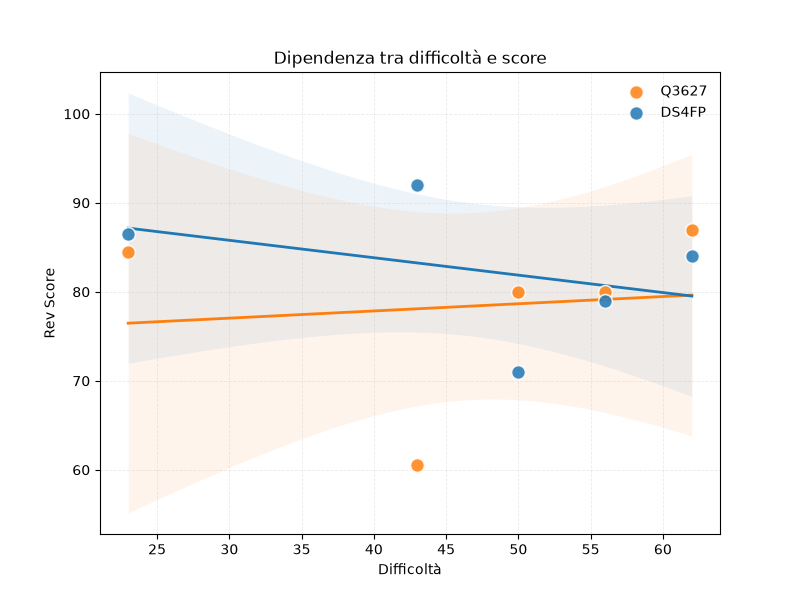
\includegraphics[scale=.75]{img/scatterplot.png}
    \caption{Dipendenza tra difficoltà e reversing}
    \label{fig:scatter_plot}
\end{figure}

\begin{equation*}
    SRE \; Success = f(Campione, Difficulty \; Score, LLM, Esecuzione)
    \label{eq:success_hypo}
\end{equation*}

Infine, è opportuno considerare le implicazioni che i risultati ottenuti hanno rispetto al livello di autonomia previsto per la pipeline di analisi. In particolare, è stato mostrato che il sistema è in grado di operare senza input umano diretto, svolgendo le attività di SRE, producendo i relativi report e proseguendo con la generazione del codice. Sebbene sia quindi tecnicamente in grado di produrre, in maniera consistente, \textsc{Capture Module} compatibili con le interfacce previste e integrabili in altri workflow, è ancora difficile e poco frequente ottenere un modulo immediatamente funzionante senza prevedere almeno un piccolo intervento iniziale di revisione o aggiustamento. I risultati suggeriscono però che l'impiego del sistema secondo un approccio \emph{human-on-the-loop} sia già concretamente praticabile, poiché il contributo richiesto all'operatore per portare a termine il processo appare contenuto. Il raggiungimento di una piena autonomia richiederebbe invece ulteriori miglioramenti, soprattutto in termini di affidabilità nell'estrazione delle informazioni e di robustezza e consistenza delle singole esecuzioni.